% Crucial Preamble
\documentclass[12pt,letterpaper]{article} \usepackage{amsmath} \usepackage{graphicx} \usepackage[margin=1in]{geometry} \usepackage{longtable}  \usepackage{amssymb}

% Extra Preamble
\usepackage{fancyhdr} \usepackage{enumitem} \usepackage{float} \usepackage{soul}
\usepackage{multicol} \usepackage[compact]{titlesec}
\usepackage{listings}
\usepackage{pdfpages}



% frames with display breaks
\usepackage{mdframed}
\allowdisplaybreaks

% change spacing
\usepackage{setspace}
\setlength{\parskip}{0.4\baselineskip}

% Remove paragraph indentation
\setlength{\parindent}{0pt}

% Reduce space before and after section headings
%\titlespacing*{\section}{0pt}{0.1\baselineskip}{0.2\baselineskip}

% changes font
%\renewcommand{\familydefault}{\sfdefault}

% adds header and footer
\pagestyle{fancy}
\fancyhead{} \fancyhead[C]{CEG 3136 Summary Sheet} \fancyhead[L]{CEG3136} \fancyhead[R]{Owen Daigle}
\fancyfoot{} \fancyfoot[C]{\thepage}

\definecolor{mygreen}{rgb}{0,0.6,0}
\definecolor{mygray}{rgb}{0.5,0.5,0.5}
\definecolor{mymauve}{rgb}{0.58,0,0.82}

\lstset{ %
	backgroundcolor=\color{white},   % choose the background color
	basicstyle=\small,        % size of fonts used for the code
	breaklines=true,                 % automatic line breaking only at whitespace
	captionpos=b,                    % sets the caption-position to bottom
	commentstyle=\color{mygreen},    % comment style
	escapeinside={<@}{@>},			 % Escapes these chars
	keywordstyle=\color{blue},       % keyword style
	stringstyle=\color{mymauve},     % string literal style
}


\begin{document}
	
	\begin{center}
		\Large\textbf{CEG 3136 Summary Sheet} \\
		\vspace{0.5em}
	\end{center}	
	
	\section{Data Representation}
	One \textbf{Byte} is defined as 8 bits. In 32 bit architecture, one \textbf{Word} is 32 bits, and therefore a half word is 16 bits, and a double word is 64 bits. 
	
	We have unsigned integers and signed integers. Unsigned is simple, signed can be represented in either signed magnitude, twos complement, or ones complement. 
	
	\begin{mdframed}
		\textbf{Ex. Show -5 in 4 bits in all 3 forms}
		
		Positive 5: \verb*|0101|
		
		Signed Magnitude: \verb*|1101|
		
		Twos Complement: \verb|1011|
		
		Ones Complement: \verb*|1010|
	\end{mdframed}
	
	In an adder/subtractor, we generate a carry flag (C) (carry out of most significant bit [MSB]) and an overflow flag (V). If we are doing unsigned, the carry flag signifies something is wrong (C=1 for addition, C=0 for subtraction). For signed, we ignore C, and use V. If V=1, something went wrong. 
	
	Overflow is the XOR of the carry out of the MSB and the carry in to the MSB. 
	
	We typically use twos complement since it makes addition and subtraction able to use the same logic. 
	
	\subsection{Strings}
	Strings are represented using \textbf{ASCII} codes. Each string is compared using its ASCII value. 
	\begin{align*}
		CAT < Cat < DOG < Dog < cat < dog
	\end{align*} 
	\begin{center}
		\begin{tabular}{|c||c|c|c|c|c|c|c|c|c|c|c|c|c|c|c|}
			\hline
			Letter & A & B & C & ... & X & Y & Z & ...  & a & b & c & ... & x & y & z \\
			\hline
			ASCII Code & 41 & 42 & 43 &  & 58 & 59 & 5A &  & 61 & 62 & 63 &  & 78 & 79 & 7A \\
			\hline
		\end{tabular}
	\end{center}
	\subsection{Fixed Point}
	The \textbf{Q Notation} represents the type of fixed point using \verb|UQm.n|. 
	\begin{center}
		\begin{tabular}{|c||c|}
			\hline
			U & Unsigned. Remove if we are doing signed \\
			\hline
			Q & Means Q notation \\
			\hline
			m & Number of integer bits \\
			\hline
			n & number of fractional bits \\
			\hline
		\end{tabular}
	\end{center}
	
	\begin{mdframed}
		\textbf{Ex. } Approximate $-\pi$ using \verb*|Q3.12|
		
		This means we have the sign bit, then 3 integer bits and 12 fractional bits. 
		
		We can represent pi as:
		\begin{align*}
			0011.001001000100
		\end{align*}
		So after taking the twos complement $- \pi$ becomes:
		\begin{align*}
			1100.110110111100
		\end{align*}
		If it was \verb*|UQ4.12| we could only represent $\pi$ not $-\pi$ but it would be:
		\begin{align*}
			0011.001001000100
		\end{align*}
	\end{mdframed}
	
	To add fixed point numbers, it is very simple. We just treat it as if the radix is non existent. 
	
	\subsection{Floating Point}
	Floating point is similar to scientific notation in decimal. We first need to normalize it. So we make it in the form of $1.xxxxxxx \times  2^{exp}$. We then hide the \verb*|1| as it is implied. 
	
	Using single precision, we have 1 bit for the sign, 8 for exponent, and 23 for the fractional. 
	
	To represent negative and positive exponents, we add 127 to the exponent. 
	
	\begin{mdframed}[]
		\textbf{Ex. } Express $(36.5625)_{10}$ as a 32 bit floating point number using the IEEE standard.
		
		The value in binary is $100100.1001$ and normalized is $1.001001001 \times 2^5$.
		
		\begin{enumerate}[noitemsep]
			\item Sign: 0
			\item Exponent: 5+127 = 132 = 10000100 
			\item Mantissa: 00100100100000000000000
		\end{enumerate}
		
		So the 32 bit number is: 0 10000100 00100100100000000000000 (without the spaces ofc)
	\end{mdframed}
	
	We reserve some values for special cases:
	\begin{center}
		\begin{tabular}{|c|c|c||c|}
			\hline
			Sign & Exponent & Fraction & Meaning \\
			\hline\hline
			1 / 0 & 0000 0000 & 0000 ... 0000 & 0 \\
			\hline
			1 / 0 & 1111 1111 & 0000 ... 0000 & + / - infinity \\
			\hline
			x & 1111 1111  & any non zero value & NaN (Not a Number) \\
			\hline
		\end{tabular}
	\end{center}
	
	Floating point has big dynamic range, but is less precise and more complicated than fixed point. 
	
	\section{ARM Instructions}
	ARM has 3 main processor families;
	\begin{center}
		\begin{tabular}{|c|l|}
			\hline
			CORTEX-A & High performance Application processors \\
			\hline
			CORTEX-R & Reliable Real time processors for mission critical purposes \\
			\hline
			CORTEX-M & Low cost, Low power Microcontroller \\
			\hline
		\end{tabular}
	\end{center}
	
	ARM has a few different instruction sets. The CORTEX-M series supports the T32 instruction set which includes both space saving 16 bit instructions, and high performance 32 bit instructions. 
	
	Other architectures such as CORTEX-A support T32 and A32 instructions with some supporting A64 as well. 
	
	ARM is a RISC architecture, so it cannot directly access memory through instructions. It must first \textbf{load} from memory into registers, then \textbf{modify}, and finally \textbf{store} back into memory.
	
	We have 16 \textbf{core registers} and some \textbf{special purpose registers }as well. Since we are 32 bit, the registers are all 32 bits wide. 
	\begin{center}
		\begin{tabular}{|c||c|l|}
			\hline
			Register & General or Special & Purpose \\
			\hline\hline
			R0 & C & General Purpose \\
			\hline
			R1 & C & General Purpose \\
			\hline
			R2 & C & General Purpose \\
			\hline
			R3 & C & General Purpose \\
			\hline
			R4 & C & General Purpose \\
			\hline
			R5 & C & General Purpose \\
			\hline
			R6 & C & General Purpose \\
			\hline
			R7 & C & General Purpose \\
			\hline
			R8 & C & General Purpose \\
			\hline
			R9 & C & General Purpose \\
			\hline
			R10 & C & General Purpose \\
			\hline
			R11 & C & General Purpose \\
			\hline
			R12 & C & Intra Procedure Call Register (IR) \\
			\hline
			R13 & C & Stack Pointer (SP) - Often there are two: \\&&MSP (Main) and PSP (Process) \\
			\hline
			R14 & C & Link Register (LR) \\
			\hline
			R15 & C & Program Counter (PC) \\
			\hline
			xPSR & S & Program Status Register \\
			\hline
			BASEPRI & S & Interrupt Priorities \\
			\hline
			PRIMASK & S & Enabling and Disabling Interrupts \\
			\hline
			FAULTMASK & S & Fault Handling \\
			\hline
			CONTROL & S &  \\
			\hline
		\end{tabular}
	\end{center}
	
	Often we map some hardware device to a memory to make it easier to work with. For example, we may have it set up so bit 7 of \verb*|R0| is 1 if an LED is on, or 0 if the LED is off. 
	
	Assembly has 4 main classes of instructions:
	\begin{itemize}
		\item Arithmetic and Logic
		\item Data Movement
		\item Compare and Branching
		\item Miscellaneous
	\end{itemize}
	
	Each instruction has 4 parts:
	\begin{center}
		\begin{tabular}{|c||l|l|l|l|}
			\hline
			General From & label & mnemonic & operand(s) & comments \\
			\hline\hline
			Ex &  & BX & LR & ; branch to LR \\
			\hline
			Ex & LOOP & CMP & R1, R2 & ; start of loop, compares R1 and R2 \\
			\hline
			Ex &  & STR & R1, R2 &  \\
			\hline
			Ex &  & ADD & R3, R5, R8 &  \\
			\hline
		\end{tabular}
	\end{center}
	
	We also have assembly directives which are just information for the assembler such as \verb*|ALIGN|, \verb*|EXPORT|, and \verb|ENDP|.
	
	\begin{center}
		\begin{tabular}{|l|l|}
			\hline
			\textbf{Directive} & \textbf{Meaning} \\
			\hline\hline
			AREA & Make a new block of data or code \\
			ENTRY & Declare an entry point where the program execution starts \\
			ALIGN & Align data or code to a particular memory boundary \\
			DCB & Allocate one or more bytes (8 bits) of data \\
			DCW & Allocate one or more half-words (16 bits) of data \\
			DCD & Allocate one or more words (32 bits) of data \\
			SPACE & Allocate a zeroed block of memory with a particular size \\
			FILL & Allocate a block of memory and fill with a given value \\
			EQU & Give a symbol name to a numeric constant \\
			RN & Give a symbol name to a register \\
			EXPORT & Declare a symbol and make it referable by other source files \\
			IMPORT & Provide a symbol defined outside the current source file \\
			INCLUDE/GET & Include a separate source file within the current source file \\
			PROC & Declare the start of a procedure \\
			ENDP & Designate the end of a procedure \\
			END & Designate the end of a source file \\
			\hline
		\end{tabular}
	\end{center}
	
	\subsection{Arithmetic and Logic}
	
	Here are just a few of the arithmetic instructions for T32.
	
	\begin{tabular}{|c|l|l|l|}
		\hline
		\textbf{Mnemonic} & \textbf{Syntax} & \textbf{Meaning} & \textbf{Operation} \\
		\hline\hline
		\textbf{ADD}   & \{Rd,\} Rn, Op2 & Add         & $\mathrm{Rd} \leftarrow \mathrm{Rn} + \mathrm{Op2}$ \\
		\textbf{ADC}   & \{Rd,\} Rn, Op2 & Add w/ carry & $\mathrm{Rd} \leftarrow \mathrm{Rn} + \mathrm{Op2} + \mathrm{Carry}$ \\
		\textbf{SUB}   & \{Rd,\} Rn, Op2 & Subtract    & $\mathrm{Rd} \leftarrow \mathrm{Rn} - \mathrm{Op2}$ \\
		\textbf{SBC}   & \{Rd,\} Rn, Op2 & Subtract w/ carry & $\mathrm{Rd} \leftarrow \mathrm{Rn} - \mathrm{Op2} + \mathrm{Carry} - 1$ \\
		\textbf{RSB}   & \{Rd,\} Rn, Op2 & Reverse subtract & $\mathrm{Rd} \leftarrow \mathrm{Op2} - \mathrm{Rn}$ \\
		\textbf{MUL}   & \{Rd,\} Rn, Rm  & Multiply      & $\mathrm{Rd} \leftarrow (\mathrm{Rn} \times \mathrm{Rm})[31:0]$ \\
		\textbf{MLA}   & Rd, Rn, Rm, Ra & \textbf{Multiply and accumulate} \\ && $\mathrm{Rd} \leftarrow (\mathrm{Ra} + (\mathrm{Rn} \times \mathrm{Rm}))[31:0]$ \\
		\textbf{MLS}   & Rd, Rn, Rm, Ra & \textbf{Multiply and subtract} \\ && $\mathrm{Rd} \leftarrow (\mathrm{Ra} - (\mathrm{Rn} \times \mathrm{Rm}))[31:0]$ \\
		\textbf{SDIV}  & \{Rd,\} Rn, Rm  & \textbf{Signed divide} & $\mathrm{Rd} \leftarrow \mathrm{Rn} \div \mathrm{Rm}$ \\
		\textbf{UDIV}  & \{Rd,\} Rn, Rm  & \textbf{Unsigned divide} & $\mathrm{Rd} \leftarrow \mathrm{Rn} \div \mathrm{Rm}$ \\
		\hline
	\end{tabular}
	
	There are also lots of logic ones such as \verb*|AND|, \verb*|ORR|, \verb*|EOR| (XOR), \verb*|ORN| (NOR) and so on.
	
	There are many other instructions, the ARM T32 instruction set has a lot. 
	
	\subsubsection{NZCV Flags}
	These flags are stored in bits 28 to 31 of the PSR. 
	
	\begin{center}
		\begin{tabular}{|c||l|}
			\hline
			Flag & Meaning \\
			\hline\hline
			N & Negative - Result is Negative \\
			\hline
			Z & Zero - Result is Zero \\
			\hline
			C & Carry - Unsigned Arithmetic out of range \\
			\hline
			V & Overflow - Signed Arithmetic out of range \\
			\hline
		\end{tabular}
	\end{center}
	
	To update these flags, we add an S to the end of the instruction. 

	\begin{mdframed}
		\textbf{Ex. }
		
		Does not update NZCV flags: ADD, SUB, MUL, etc
		
		Does update NZCV flags: ADDS, SUBS, MULS, etc
		
		Always updates NZCV flags: CMP, CMN, TST, TEQ
	\end{mdframed}

	
	
	\subsubsection{Saturation}
	Saturation is a logical operation that deals with the case where overflow occurs. 
	
	Normally, it will wrap back around to the lowest value. However, sometimes we want to cap the highest value. 
	
	\begin{center}
		\begin{tabular}{|c|c|}
			\hline
			With Saturation (4 bits) & 7+1=-8 \\
			\hline
			Without Saturation (4 bits) & 7+1=7 \\
			\hline
		\end{tabular}
	\end{center}
	
	\begin{figure}[h!]
		\centering
		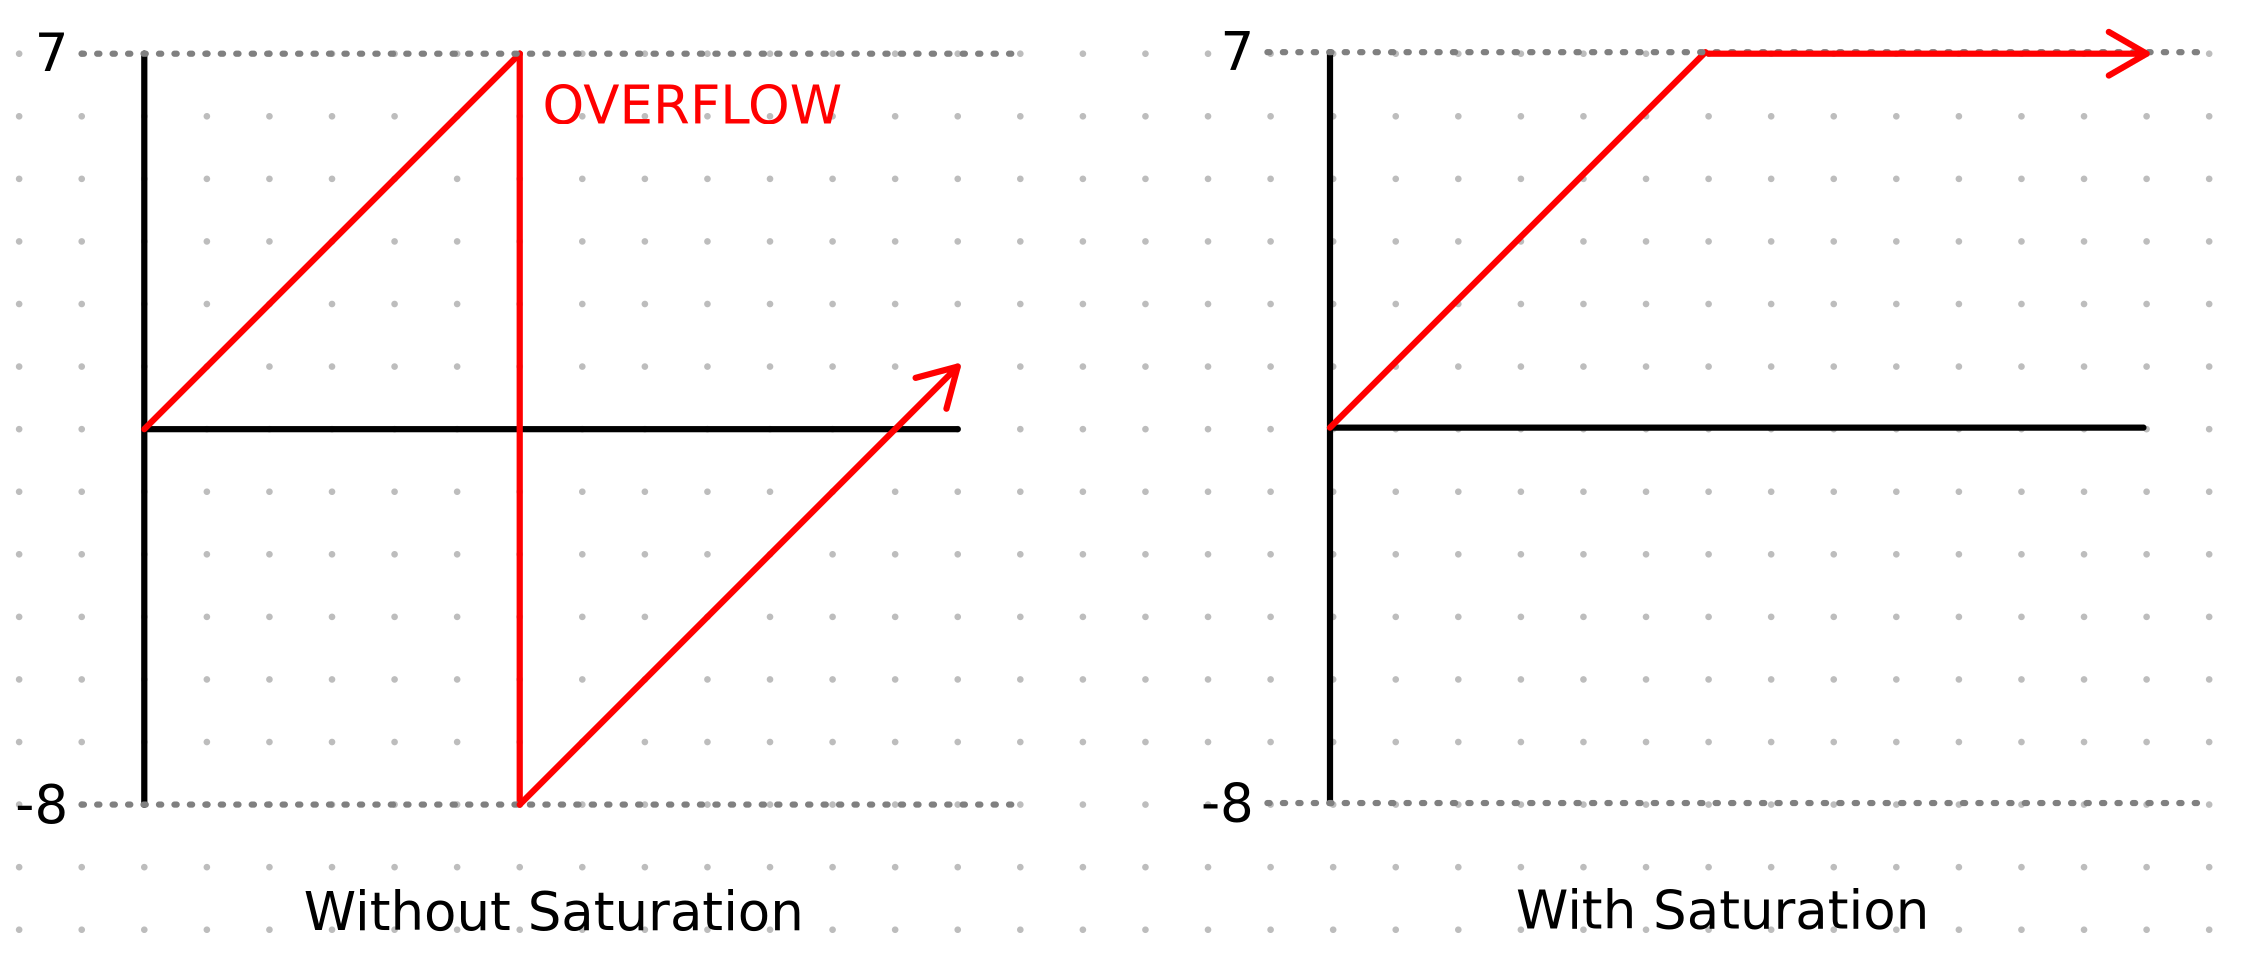
\includegraphics[width=0.7\linewidth]{images/saturation}
		\caption{Saturation}
		\label{fig:saturation}
	\end{figure}
	
	\subsubsection{Other Instructions}
	
	\begin{center}
		\begin{tabular}{|c|c|p{7cm}|}
			\hline
			Instruction & Description & Similar Instructions \\
			\hline\hline
			RBIT Rd, Rn & Reverses bit order in word & REV (byte order), REV16 (For half words), REVSH (Sign Extend) \\
			\hline
			SXTB \{Rd,\} Rm & Sign Extension (Byte) & SXTH (Half word), UXTB/UXTH (Zero extend) \\
			\hline
			MOV Rd, Rx & Move from Rx to Rd & MVN (MV and NOT), MRS (From special reg), MSR (From gen to special) \\
			\hline
			LSL Rd, Rn, \# & Move Rn to Rd and left shift & LSR (right logical), ASR (Right arithmetic), ROR (rotate right) \\
			\hline
		\end{tabular}
	\end{center}
	
	
	\subsection{Memory}
	Memory is byte addressable, but we typically only start a 32 bit word at a multiple of 4, a 16 bit half word at a multiple of 2, and a byte at any point. 
	
	\begin{center}
		\begin{tabular}{|c|c|}
			\hline
			LDRxx R0, [R1] & Load from memory at R1 into R0 \\
			\hline
			STRxx R0, [R1] & Store contents of R0 into memory at R1 \\
			\hline
		\end{tabular}
	\end{center}
	
	If we are storing something smaller than the memory width (byte, or halfword) we need to differentiate between signed (add \verb*|S|) [\verb*|LDRSB|, \verb*|LDRSH|] and unsigned (do not add \verb|S|) [\verb*|LDRB|, \verb*|LDRH|].
	
	When loading and storing, we can also address bits after the location we specify. This is useful for arrays. We have a few modes:
	\begin{center}
		\begin{tabular}{|c|c|l|}
			\hline
			Register Offset & LDR r0, [r1, r2] & Target: r1+r2 \\
			\hline
			Immidiate Offset & LDR r0, [r1, \#8] & Target: r1 + 8 \\
			\hline
			Pre-Index & LDR r0, [r1, \#4]! & Target: r1+4, update r1 to r1+4 after read \\
			\hline
			PostIndex & LDR r0, [r1], \#4 & Target: r1, increase r1 by 4 after read \\
			\hline
		\end{tabular}
	\end{center}
	
	\subsection{Endianess}
	Endianess means within a 32 bit word (or any multi byte data structure) do we start the LSB at the low address (little endian) or high address (big endian)?
	
	\begin{figure}[h!]
		\centering
		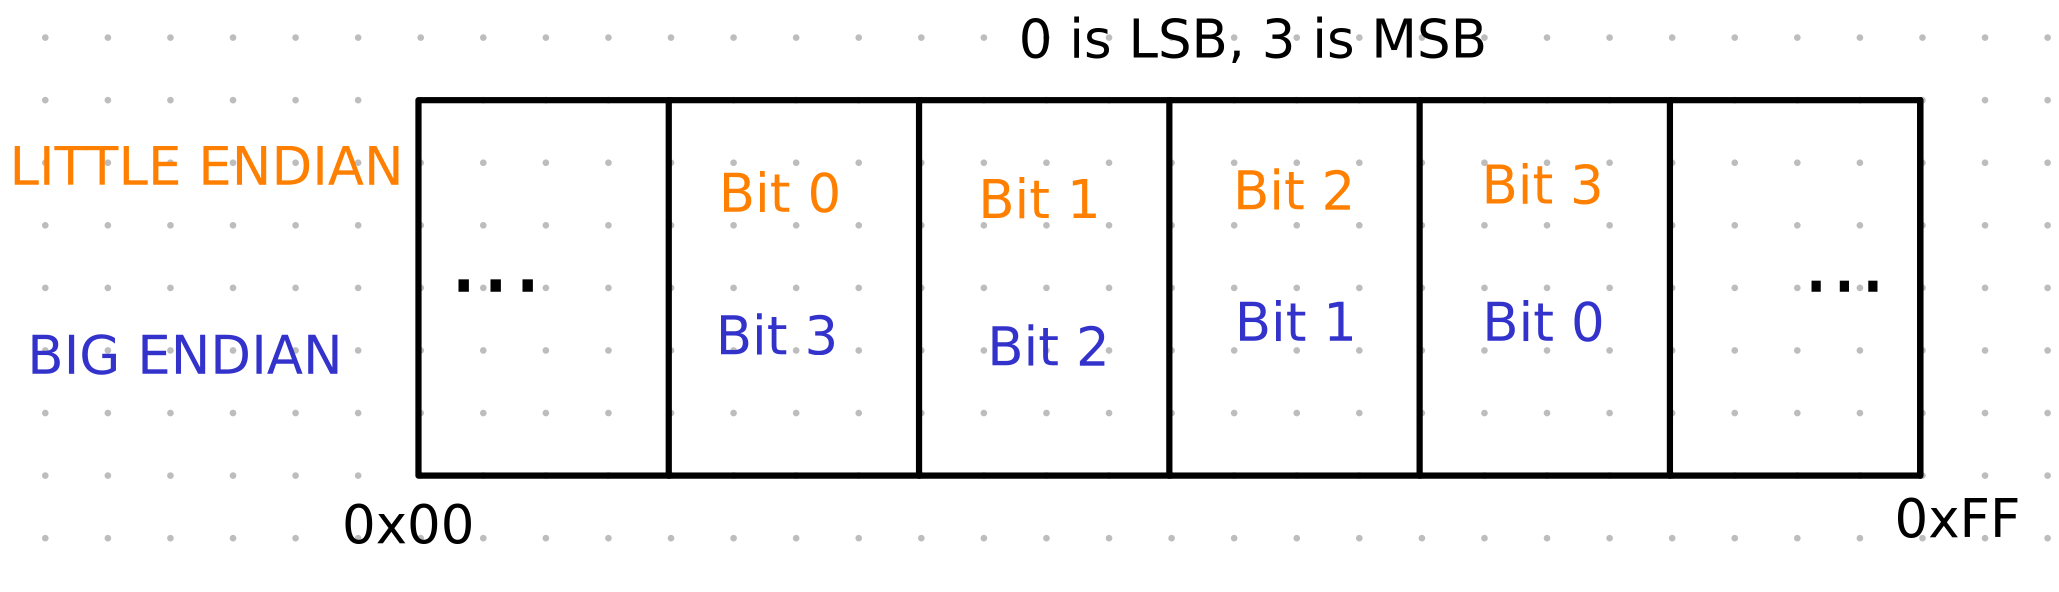
\includegraphics[width=0.5\linewidth]{images/endian}
		\caption{Endianess}
		\label{fig:endian}
	\end{figure}
	
	\subsection{Control Flow Instructions}
	We have 4 variations of the branch command. These will branch to either a label, or an address. 
	\begin{center}
		\begin{tabular}{|c|c|c|}
			\hline
			Instruction & Operands & Description \\
			\hline\hline
			B & label & Branch \\
			\hline
			BL & label & Branch with link \\
			\hline
			BLX & Rm & Branch and Exchange with link \\
			\hline
			BX & Rm & Branch and Exchange \\
			\hline
		\end{tabular}
	\end{center}
	
	We have condition codes. These are appended to almost any instruction and they will only execute the instruction if the condition is true. It uses the status flags NZCV. These are typically performed after a \verb|CMP| operation.
	\begin{center}
		\begin{tabular}{|l|l|l|}
			\hline
			Suffix & Description & Flags tested \\
			\hline
			EQ    & Equal                       & $Z = 1$ \\
			NE    & Not Equal                   & $Z = 0$ \\
			CS/HS & Unsigned Higher or Same     & $C = 1$ \\
			CC/LO & Unsigned Lower              & $C = 0$ \\
			MI    & Minus (Negative)            & $N = 1$ \\
			PL    & Plus (Positive or Zero)     & $N = 0$ \\
			VS    & Overflow Set                & $V = 1$ \\
			VC    & Overflow Cleared            & $V = 0$ \\
			HI    & Unsigned Higher             & $C = 1 \ \&\ Z = 0$ \\
			LS    & Unsigned Lower or Same      & $C = 0 \ \mid\ Z = 1$ \\
			GE    & Signed Greater or Equal     & $N = V$ \\
			LT    & Signed Less Than            & $N \neq V$ \\
			GT    & Signed Greater Than         & $Z = 0 \ \&\ N = V$ \\
			LE    & Signed Less than or Equal   & $Z = 1 \ \mid\ N \neq V$ \\
			AL    & Always                      & None \\
			\hline
		\end{tabular}
		
	\end{center}
	\begin{mdframed}
		\textbf{Ex.} Branch to \verb*|FOO| if \verb*|r0| is less than \verb*|0|.
		\begin{lstlisting}
CMP r0, #0		;compare r0 with 0
BLE FOO 		;branch to FOO if LE (Z=1)
		\end{lstlisting}
		
		This is similar to some c code doing:
		\begin{lstlisting}[language=c]
if (a < 0) { //assuming a is in r0
	foo(); //or something else, whatever code is located at FOO
}
		\end{lstlisting}
	\end{mdframed}
	
	ARM assembly lets us use the IT (If Then) syntax as well. 
	\begin{mdframed}
		\textbf{Ex.} 
		\begin{lstlisting}
ITTE NE			; Two commands will follow with NE
ANDNE r0, r0, r1	; Then one command with the opposite
ANDNE r2, r2, #1	; of NE which is EQ
MOVEQ r2, r3		;

ITT EQ			; The IT can be ommitted from code
MOVEQ ...		; and the assembler will add it.
ADDEQ ...
		\end{lstlisting}
	\end{mdframed}
	
	\section{Subroutines}
	The link register \verb*|LR| contains the return address of the subroutine. This is copied back to the PC when the subroutine is finished. 
	
	In ARM, we store any parameters in registers R0 through R3. Any additional parameters need to be put on the stack. Also, if the parameters are larger than 32 bits, they can take up more than one register (a 128 bit parameter would take up R0, R1, R2, R3).
	
	It returns the return value in R0.
	
	Registers R0 through R3 can be freely changed by the subroutine, as well as R12 and R14 (LR). In other words, the calling function cannot expect them to keep the same data when the subroutine returns. The opposite is true with registers R4 to R11 where they must be preserved. If the subroutine changes anything in those registers, it must return them to the previous value before returning. 
	
	We use \verb*|BL| or \verb*|BLX| to call a subroutine. 
	
	\subsection{Stack}
	The ARM stack uses a full descending stack. This means that the stack pointer points to the top piece of data on the stack. The stack also grows down to memory address 0 as items are pushed to it. 
	
	We have the instructions \verb*|PUSH <reg list>| and \verb*|POP <reg list>|. 
	
	When we push or pop multiple registers, the highest number register is pushed first, and popped last. 
	
	\begin{mdframed}
		\textbf{Ex.} \verb*|PUSH {r6, r8, r7}|
		
		This instruction will first push \verb|r8|, followed by \verb*|r7| and then finally \verb*|r6|.
		
		It would be equivalent to \verb*|PUSH {r6, r7, r8}| and to \verb*|PUSH {r8, r6, r7}| and so on.
	\end{mdframed}
	
	\begin{mdframed}
		\textbf{Ex.} \verb*|POP {r6, r8, r7}|
		
		This instruction will first pop \verb|r6|, followed by \verb*|r7| and then finally \verb*|r8|.
		
		It would be equivalent to \verb*|POP {r6, r7, r8}| and to \verb*|POP {r8, r6, r7}| and so on.
	\end{mdframed}
	
	\begin{mdframed}
		\textbf{Ex.}
		\begin{lstlisting}
...			;main program
	BL foo
...

foo PROC
	PUSH {r4}	;we are using r4 which must be preserved
	...
	MOV r4, #1	;this changes r4, good thing we saved it
	...
	POP {r4}	;this restores r4 for the caller function
	BX LR		;goes back to caller
ENDP
		\end{lstlisting}
	\end{mdframed}
	
	We also need to preserve the LR on the stack if we call a subroutine from inside a subroutine since it could be overridden. Then we would have no way to return to the main program.
	
	Often we have two stack pointers, the \verb*|MSP| (main) and \verb*|PSP| (process). This is toggled by a bit in the CONTROL register. 
	
	\section{C and Assembly}
	When we have C code, it goes through a lot of steps to get into ARM assembly to be loaded onto the microcontroller.
	\begin{align*}
		Proprocessor \to Compiler \to Assembler \to Linker \to Loader \to MCU (thru \text{ }programmer)\\\to Debugger
	\end{align*}
	
	Typically, C will set up data so every word starts at an even multiple of 4 bits address. This is for efficiency. Same idea with half words, but every 2 bits. C does this by padding extra space. We can use the \verb*|__packed| keyword in c to not pad the extra space. But this can cause weird behavior. 
	
	If we want to mix C and assembly, we can do this. In assembly, we call a C function using the \verb*|import| keyword, and export a function to C using the \verb*|export| keyword. Similarly, in C we can import something from assembly using the \verb*|extern| keyword. This can work with data as well as functions. 
	
	\subsection{Volatile Datatypes}
	The \verb|volatile| keyword means each time we use a variable, we need to import it from memory into a register. This is useful when an external event may change memory at any point. In this case, we need to ensure that we don't use an old version of the variable.
	
	\subsection{Interrupts}
	An interrupt is a signal that occurs that tells the controller that it needs to stop whatever it is currently doing, save the state using the stack, and then move on to the interrupt service routine (ISR). After it then restores the stack, and goes back to the user program.
	
	It needs to save \verb*|xPSR|, \verb*|PC|, \verb*|LR|, \verb*|R12|, \verb*|R3|, \verb*|R2|, \verb*|R1|, and \verb*|R0| . Therefore it can use any of those registers to store data. Any other registers that are used must be returned to their original state. 
	
	\newpage 
	\section{Appendix}
	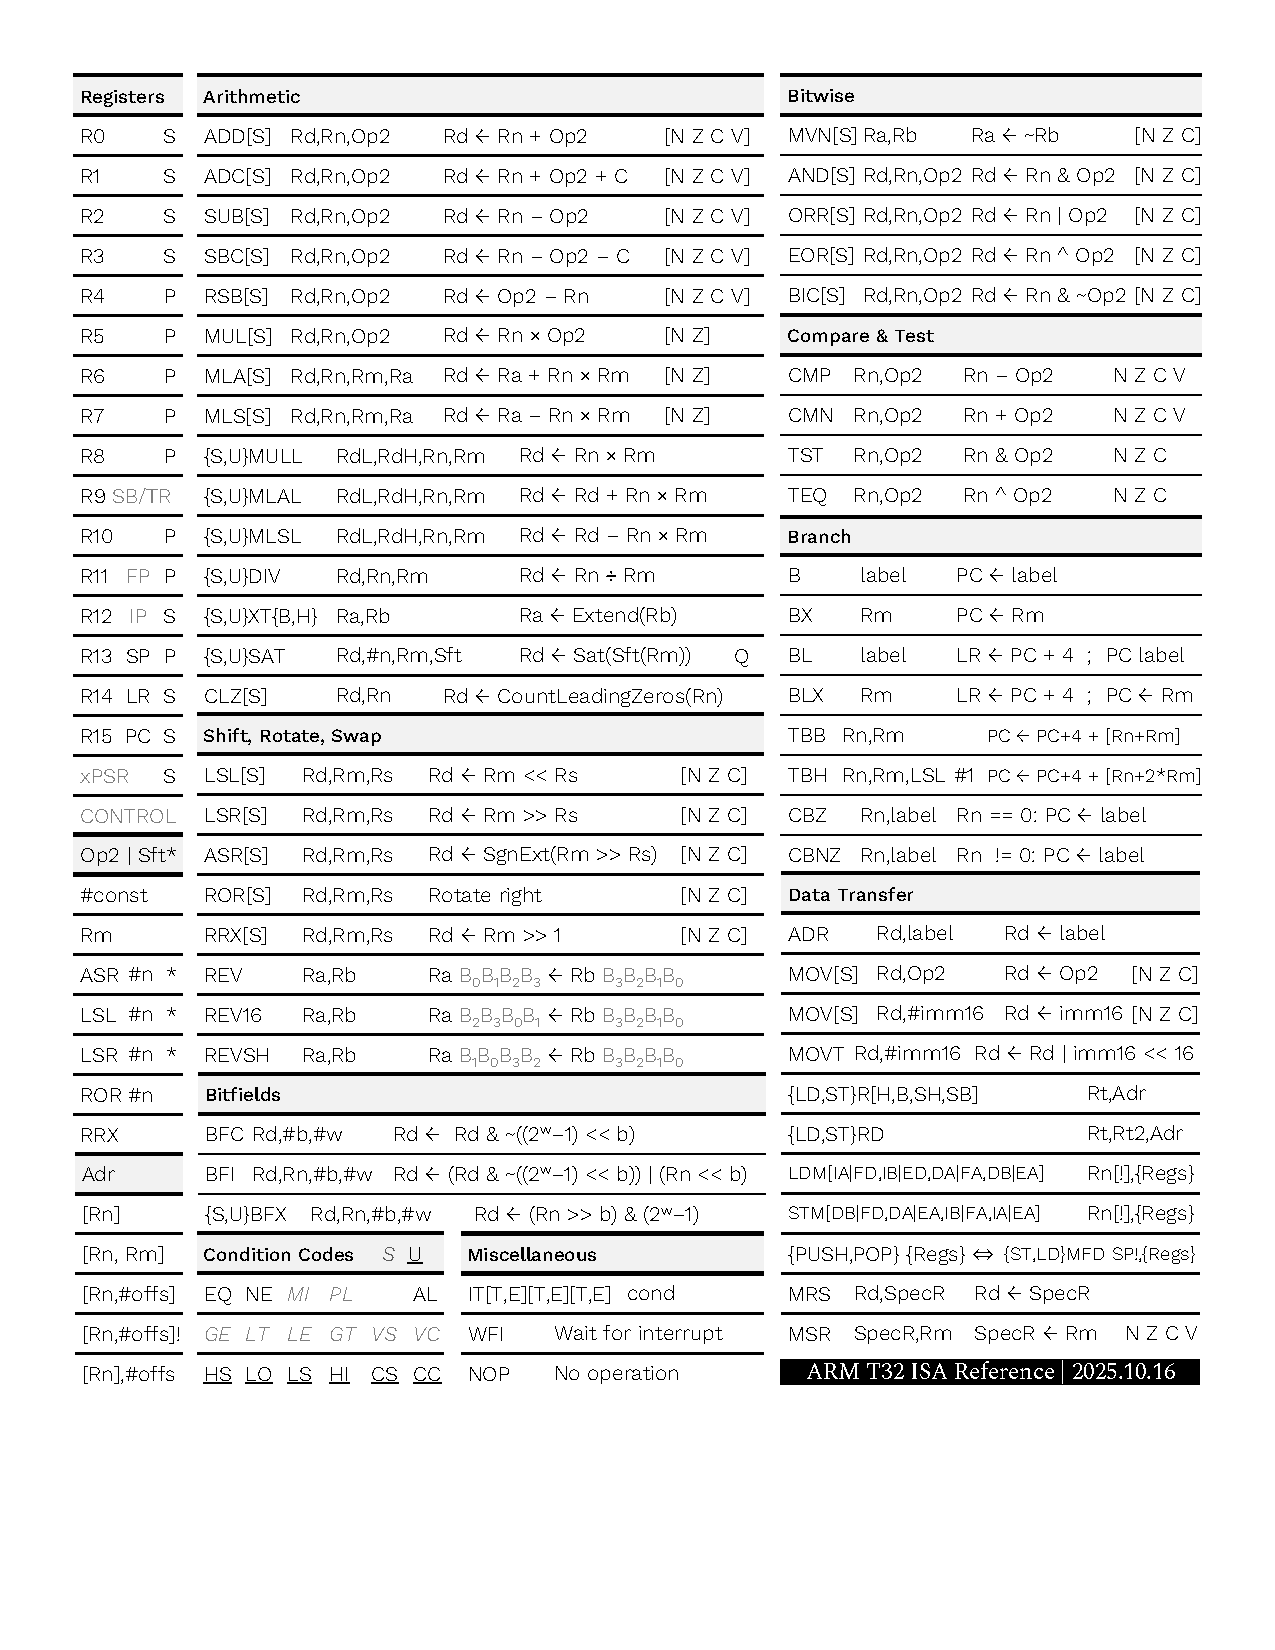
\includepdf[pages=-]{arm_reference_sheet.pdf}
	
	
	
	
\end{document}